\chapter{Metodolog\'ia}

\label{Chapter3}

En este cap\'itulo se detallar\'an los procesos abordados para la extracci\'on y clasificaci\'on de los d\'igitos
escritos en los telegramas de las elecciones.

\section{Extracci\'on, transformaci\'on y carga de d\'igitos de los telegramas}

Los telegramas de las elecciones de Santa Fe presentan un formato tabular, donde cada fila representa un partido
pol\'itico y los votos obtenidos abiertos por senadores y diputados. Se debieron ejecutar m\'ultiples pasos de
extracci\'on, transformaci\'on y carga (ETL por sus siglas) de los mismos antes de poder armar un dataset con el cual
entrenar los modelos. Se utiliz\'o la librer\'ia OpenCV \parencite{opencv_library} para manipular las im\'agenes y poder llevar a cabo el proceso de ETL.

\subsection{Enderezado}
Como los telegramas son escaneados a mano, el primer paso consiste en enderezarlos. Este proceso puede realizarse
buscando el rect\'angulo de mayor \'area, calculando el \'angulo de rotaci\'on y rotando la imagen completa con la
funci\'on \verb|getRotationMatrix2D| de OpenCV.

\begin{figure}[H]
    \centering

    \tikzset{every picture/.style={line width=0.75pt}}

    \begin{tikzpicture}[x=0.75pt,y=0.75pt,yscale=-1,xscale=1]

        \draw (370,140) node  {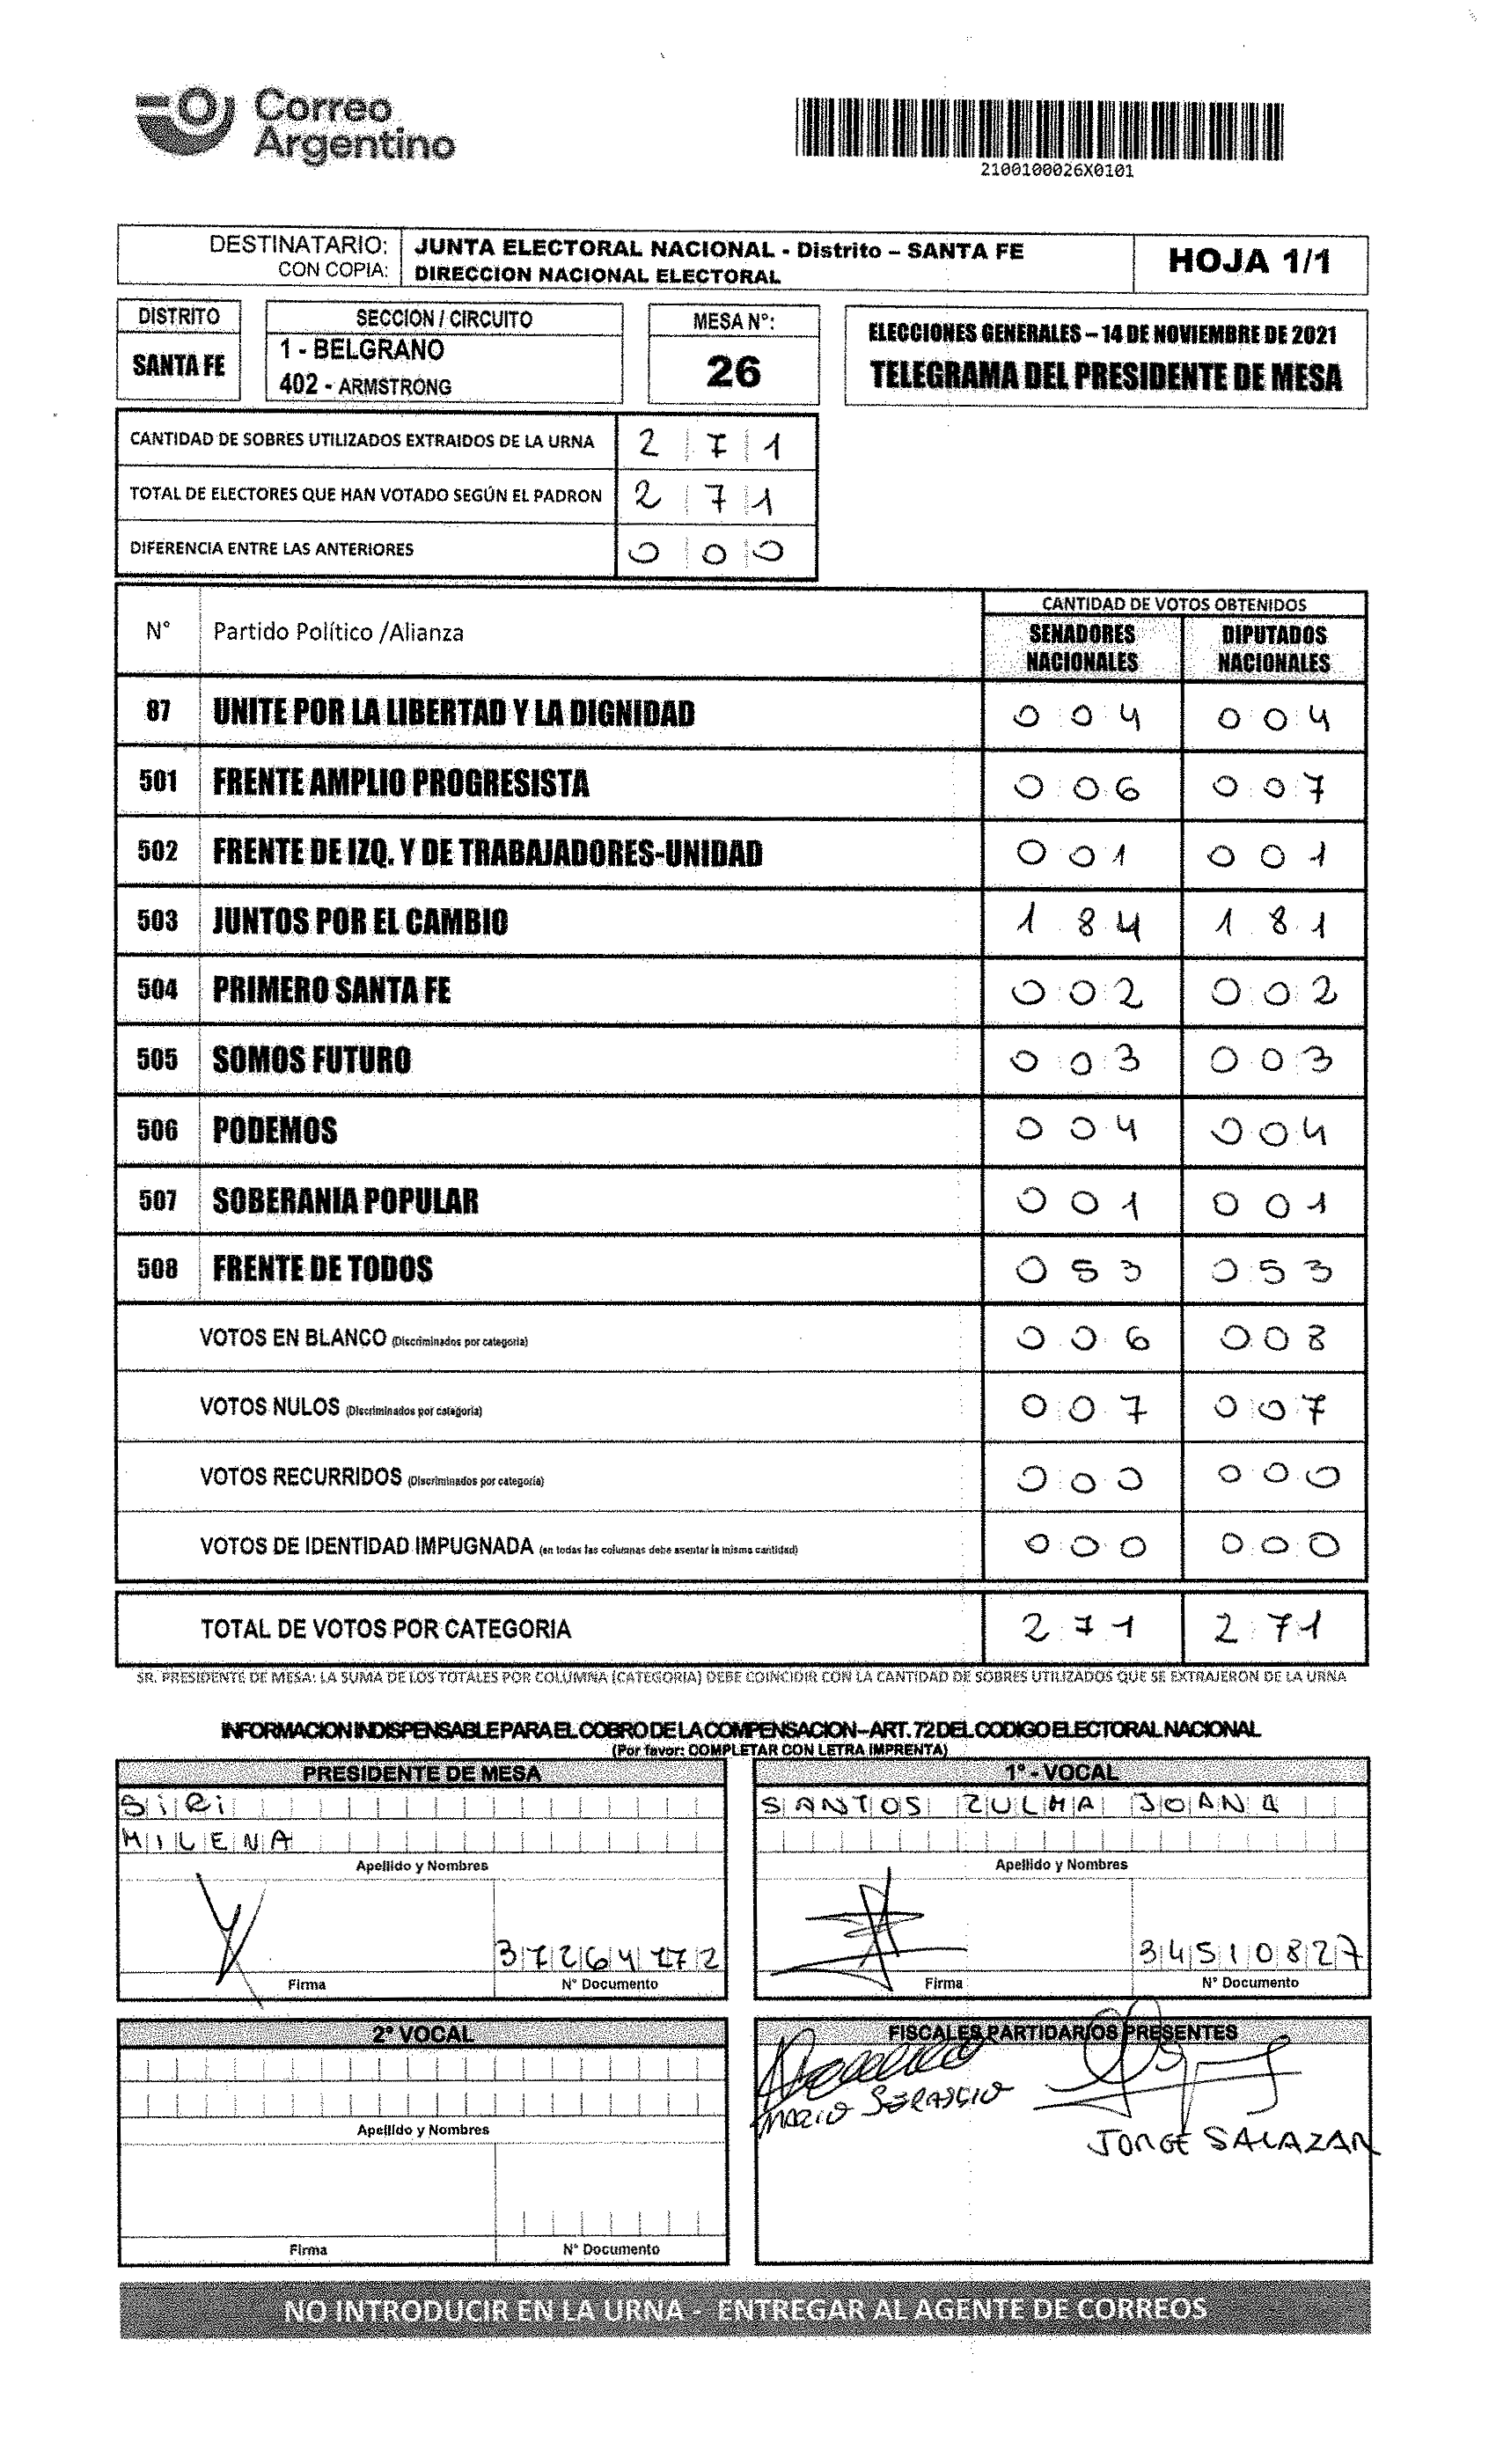
\includegraphics[width=135pt,height=210pt]{chapter3/etl-2-rotacion.png}};
        \draw (90,140) node  {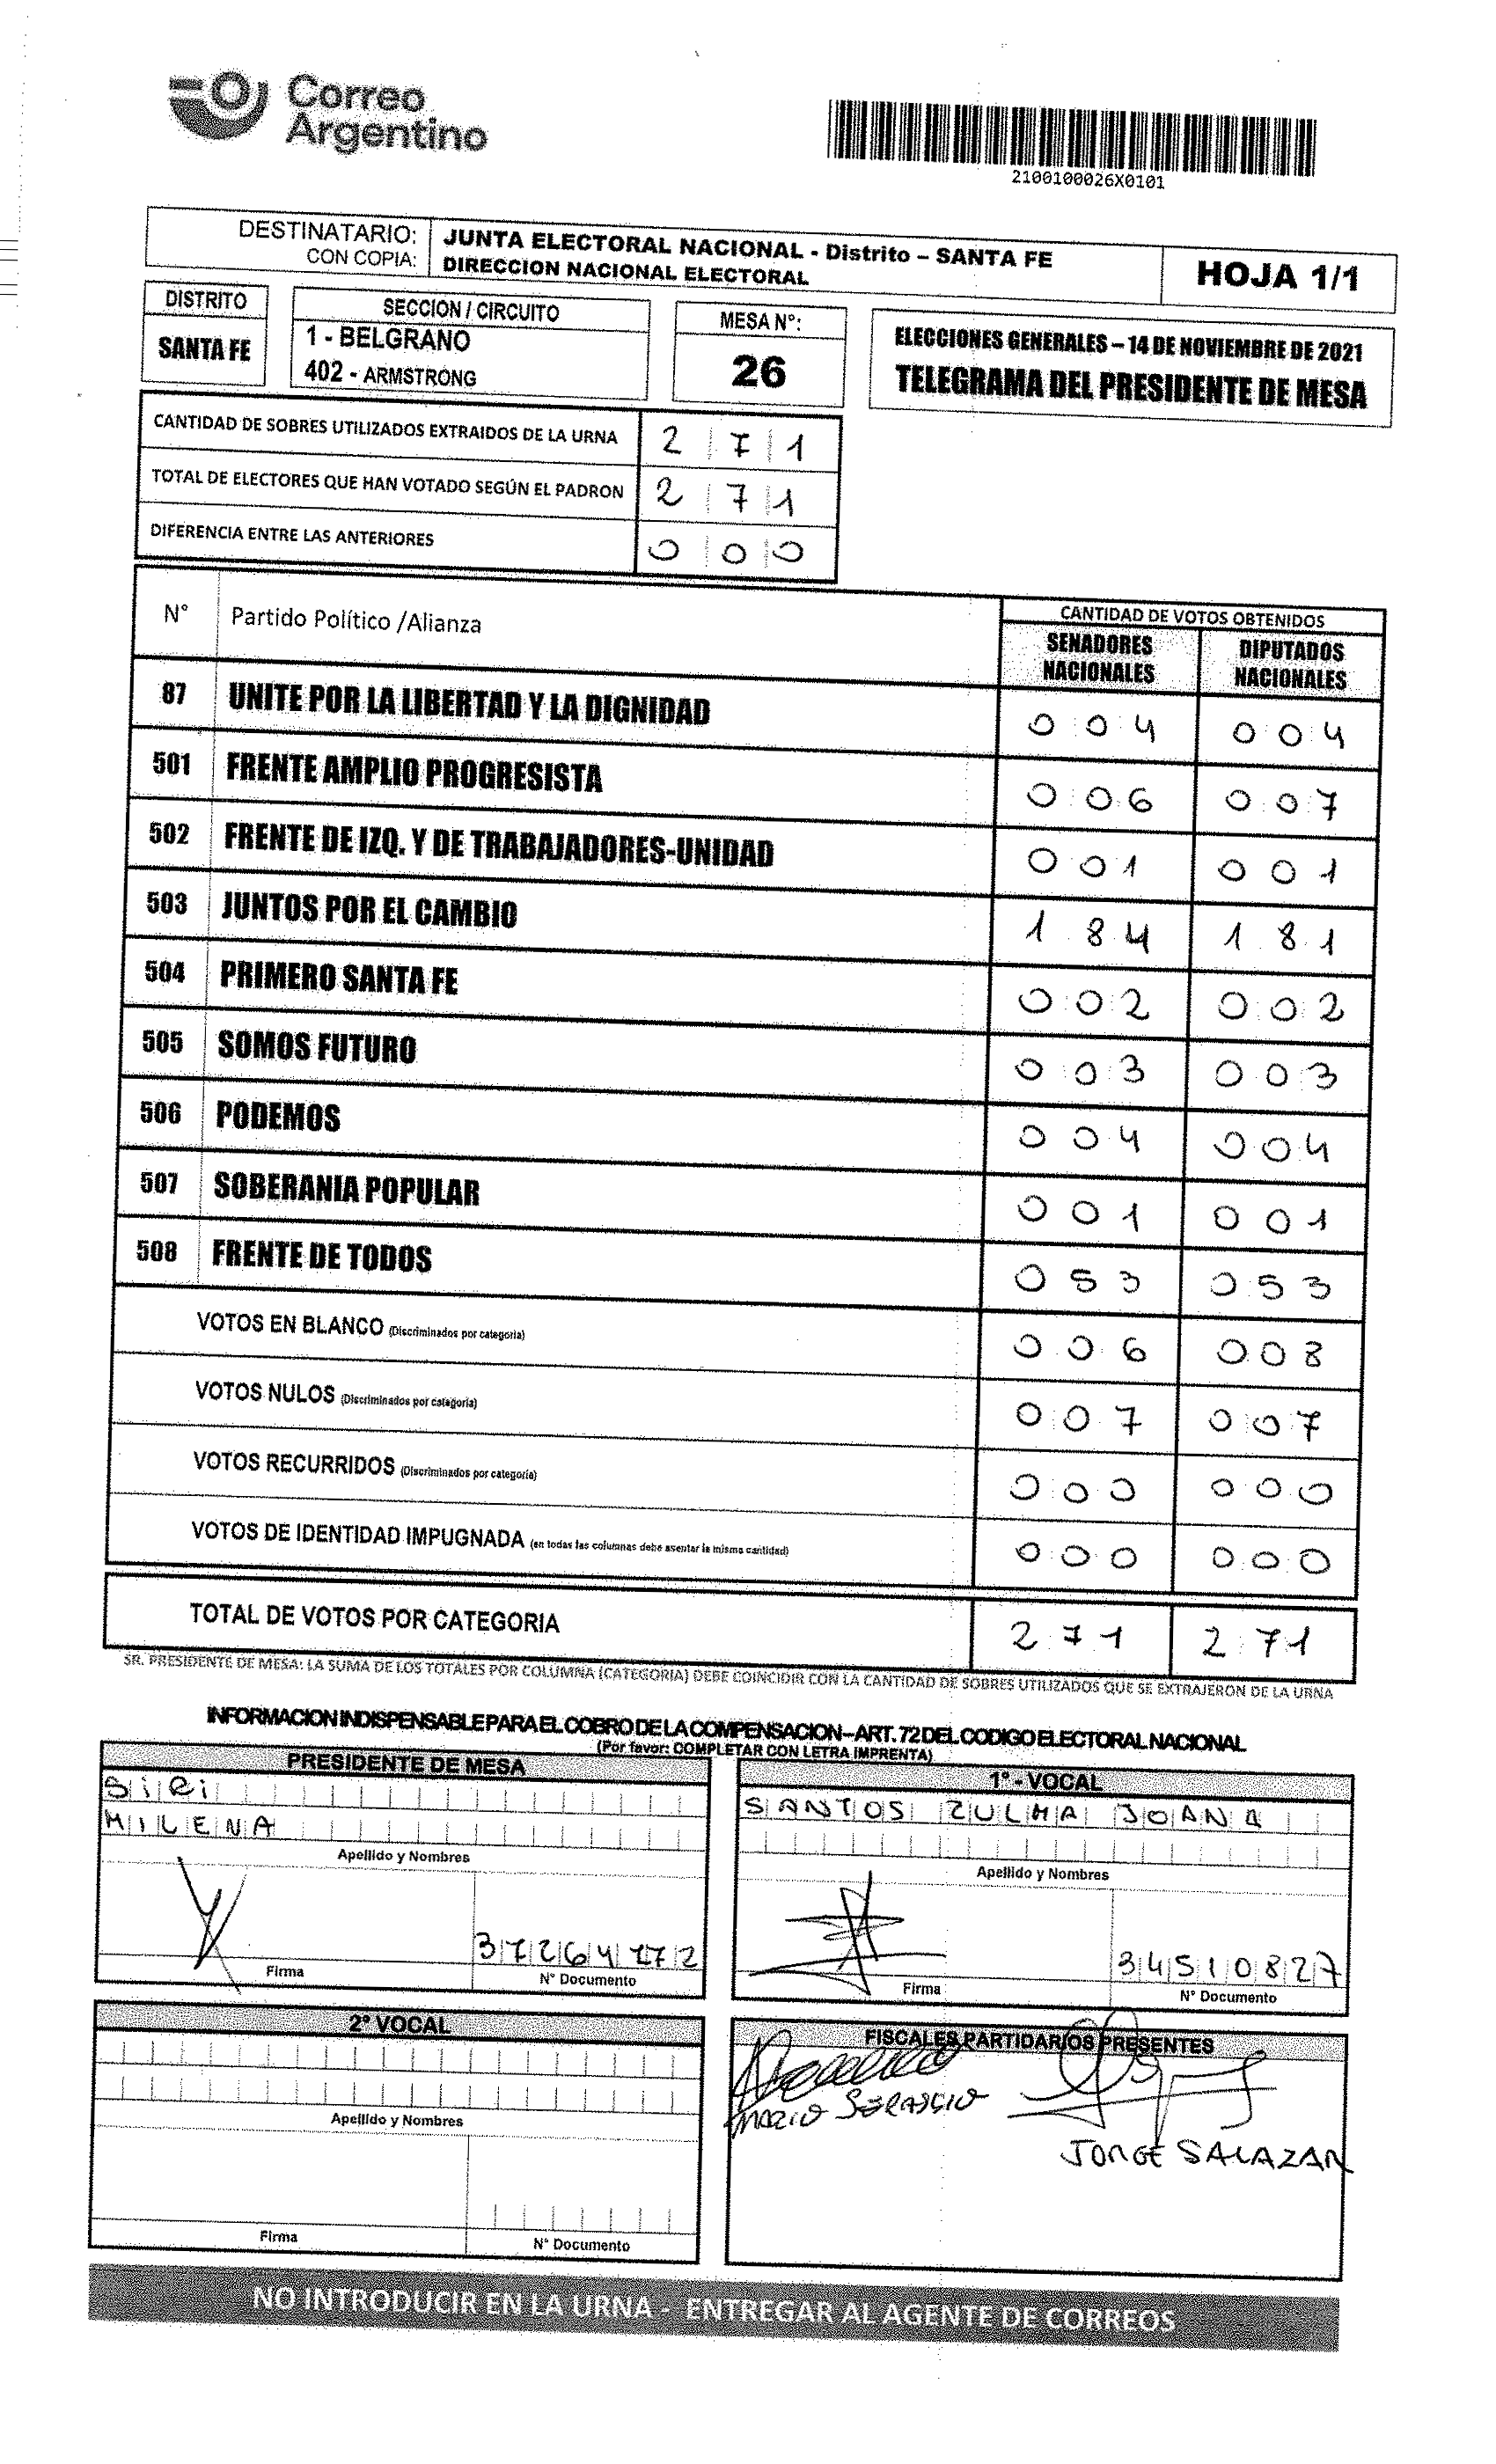
\includegraphics[width=135pt,height=210pt]{chapter3/etl-1-telegrama.png}};
        \draw    (190.8,110.6) -- (267.4,110.6) ;
        \draw [shift={(269.4,110.6)}, rotate = 180] [color={rgb, 255:red, 0; green, 0; blue, 0 }  ][line width=0.75]    (10.93,-3.29) .. controls (6.95,-1.4) and (3.31,-0.3) .. (0,0) .. controls (3.31,0.3) and (6.95,1.4) .. (10.93,3.29)   ;
        \draw (190,87.18) node [anchor=north west][inner sep=0.75pt]   [align=left] {Enderezar};

    \end{tikzpicture}

    \caption{Enderezamiento de un telegrama utilizando OpenCV.}
    \label{fig:etl-1-rotacion}
\end{figure}

\subsection{Extracci\'on de la grilla de votos}
El siguiente paso consiste en poder seleccionar la grilla de los votos y poder extraerla para seguir trabajando en
ella.

\section{Modelo baseline}

\lipsum[1]

\section{Adaptaci\'on de dominio}

\lipsum[1]

\subsection{DANN}

\lipsum[1]

\subsection{ADDA}

\lipsum[1]

\subsection{AFN}

\lipsum[1]

\subsection{MDD}

\lipsum[1]
